\documentclass[11pt,a4paper]{report}

% =============================================================================
% PACKAGES
% =============================================================================
\usepackage[utf8]{inputenc}
\usepackage[T1]{fontenc}
\usepackage{amsmath,amssymb,amsfonts}
\usepackage{mathtools}
\usepackage{bm}
\usepackage{graphicx}
\usepackage{booktabs}
\usepackage{longtable}
\usepackage{array}
\usepackage{multirow}
\usepackage{xcolor}
\usepackage{listings}
\usepackage{algorithm}
\usepackage{algpseudocode}
\usepackage{hyperref}
\usepackage{geometry}
\usepackage{fancyhdr}
\usepackage{titlesec}
\usepackage{tocloft}
\usepackage{nomencl}
\usepackage{siunitx}
\usepackage{tikz}
\usetikzlibrary{shapes,arrows,positioning,calc,fit,backgrounds}

\geometry{margin=2.5cm}
\hypersetup{
    colorlinks=true,
    linkcolor=blue!70!black,
    citecolor=green!50!black,
    urlcolor=blue!70!black
}

% =============================================================================
% CODE LISTING STYLE
% =============================================================================
\definecolor{codegreen}{rgb}{0,0.6,0}
\definecolor{codegray}{rgb}{0.5,0.5,0.5}
\definecolor{codepurple}{rgb}{0.58,0,0.82}
\definecolor{backcolour}{rgb}{0.97,0.97,0.97}

\lstdefinestyle{pythonstyle}{
    backgroundcolor=\color{backcolour},
    commentstyle=\color{codegreen},
    keywordstyle=\color{blue},
    numberstyle=\tiny\color{codegray},
    stringstyle=\color{codepurple},
    basicstyle=\ttfamily\footnotesize,
    breakatwhitespace=false,
    breaklines=true,
    captionpos=b,
    keepspaces=true,
    numbers=left,
    numbersep=5pt,
    showspaces=false,
    showstringspaces=false,
    showtabs=false,
    tabsize=2,
    language=Python
}
\lstset{style=pythonstyle}

% =============================================================================
% CUSTOM COMMANDS
% =============================================================================
\newcommand{\vecbold}[1]{\boldsymbol{#1}}
\newcommand{\mat}[1]{\mathbf{#1}}
\newcommand{\transpose}{^{\mathsf{T}}}
\newcommand{\inv}{^{-1}}
\newcommand{\ztd}{\mathrm{ZTD}}
\newcommand{\zhd}{\mathrm{ZHD}}
\newcommand{\zwd}{\mathrm{ZWD}}
\newcommand{\iwv}{\mathrm{IWV}}
\newcommand{\ppp}{\mathrm{PPP}}
\newcommand{\ar}{\mathrm{AR}}

% =============================================================================
% DOCUMENT INFO
% =============================================================================
\title{
    \vspace{-2cm}
    \Huge\textbf{PyGNSS-RT Technical Design Document}\\[0.5cm]
    \Large Python-Based Real-Time PPP-AR GNSS Positioning System\\[0.3cm]
    \large Comprehensive Technical Specification and Implementation Guide
}
\author{
    \textbf{GNSS Research Group}\\
    Institute for Earth Sciences and Space Geodesy\\[0.3cm]
    \texttt{pygnss\_rt v1.4.0}
}
\date{\today}

% =============================================================================
% BEGIN DOCUMENT
% =============================================================================
\begin{document}

\maketitle

\begin{abstract}
This document provides a comprehensive technical specification for the \texttt{pygnss\_rt} Python package, a production-grade framework for Real-Time Precise Point Positioning with Ambiguity Resolution (PPP-AR). The system integrates with the Bernese GNSS Software v5.4 for core geodetic computations while providing a sophisticated Python orchestration layer for data management, product acquisition, and operational automation. This document covers the complete system architecture, mathematical foundations of PPP-AR, advanced error modeling including VMF3 tropospheric mapping functions and Observation Specific Biases (OSB), the LAMBDA-based ambiguity resolution strategy, and detailed Python implementation patterns. The system supports multi-GNSS processing (GPS, GLONASS, Galileo, BeiDou) with sub-centimeter positioning accuracy under favorable conditions.
\end{abstract}

\tableofcontents
\listoffigures
\listoftables

% =============================================================================
% CHAPTER 1: INTRODUCTION
% =============================================================================
\chapter{Introduction}

\section{Document Purpose and Scope}

This technical design document serves as the authoritative reference for the \texttt{pygnss\_rt} real-time GNSS processing system. It provides:

\begin{itemize}
    \item Complete mathematical formulations for PPP-AR processing
    \item Detailed system architecture and data flow specifications
    \item Implementation details for atmospheric and bias modeling
    \item Ambiguity resolution algorithms and validation strategies
    \item Python code structure and optimization techniques
\end{itemize}

\section{System Overview}

The \texttt{pygnss\_rt} package implements a sophisticated orchestration framework for GNSS data processing, designed for:

\begin{enumerate}
    \item \textbf{Near Real-Time (NRT) Operations}: Hourly and sub-hourly processing with configurable latencies
    \item \textbf{Multi-GNSS Support}: GPS (G), GLONASS (R), Galileo (E), and BeiDou (C) constellations
    \item \textbf{PPP-AR Processing}: Integer ambiguity resolution using CODE products
    \item \textbf{Atmospheric Monitoring}: ZTD estimation and IWV derivation for meteorology
    \item \textbf{Network Processing}: Five international networks (IGS, EUREF, GB, RGP, Supersites)
\end{enumerate}

\section{Key Capabilities}

\begin{table}[h]
\centering
\caption{PyGNSS-RT System Capabilities}
\label{tab:capabilities}
\begin{tabular}{lll}
\toprule
\textbf{Feature} & \textbf{Implementation} & \textbf{Status} \\
\midrule
PPP-AR Processing & CODE products + BSW & Operational \\
Multi-GNSS (GRE) & GPS+GLONASS+Galileo & Operational \\
VMF3 Troposphere & TU Wien grids & Operational \\
OSB/BIA Handling & CODE signal biases & Operational \\
Hourly Processing & 3-hour latency & Operational \\
Sub-hourly (15-min) & Climate research & Operational \\
IWV Generation & Bevis formulation & Operational \\
\bottomrule
\end{tabular}
\end{table}

% =============================================================================
% CHAPTER 2: SYSTEM ARCHITECTURE
% =============================================================================
\chapter{System Architecture and Data Flow}

\section{Architectural Overview}

The \texttt{pygnss\_rt} system follows a modular pipeline architecture with clear separation of concerns:

\begin{figure}[h]
\centering
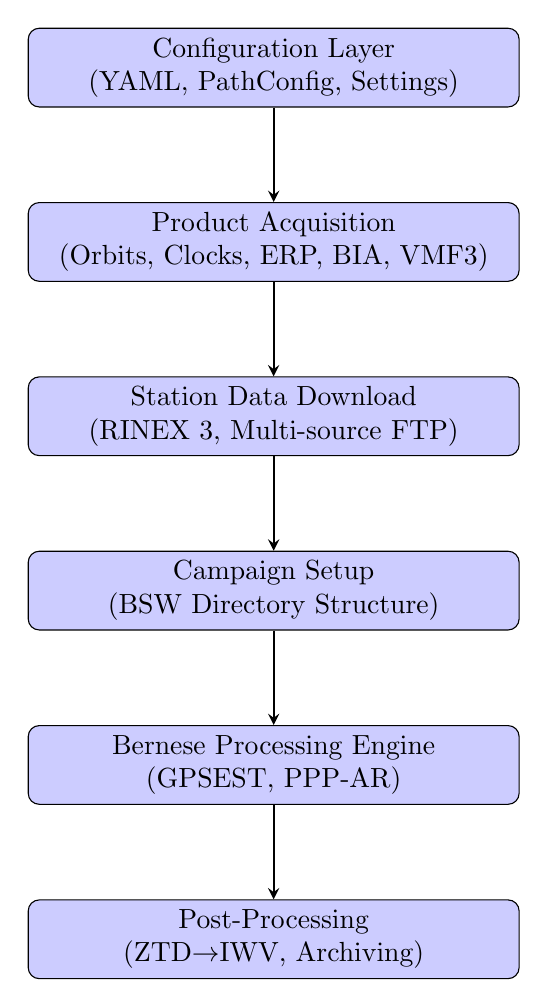
\begin{tikzpicture}[
    node distance=1.2cm,
    block/.style={rectangle, draw, fill=blue!20, text width=6cm, text centered, rounded corners, minimum height=1cm},
    arrow/.style={->, thick, >=stealth}
]
    % Nodes
    \node[block] (config) {Configuration Layer\\(YAML, PathConfig, Settings)};
    \node[block, below=of config] (products) {Product Acquisition\\(Orbits, Clocks, ERP, BIA, VMF3)};
    \node[block, below=of products] (stations) {Station Data Download\\(RINEX 3, Multi-source FTP)};
    \node[block, below=of stations] (campaign) {Campaign Setup\\(BSW Directory Structure)};
    \node[block, below=of campaign] (bsw) {Bernese Processing Engine\\(GPSEST, PPP-AR)};
    \node[block, below=of bsw] (postproc) {Post-Processing\\(ZTD$\rightarrow$IWV, Archiving)};

    % Arrows
    \draw[arrow] (config) -- (products);
    \draw[arrow] (products) -- (stations);
    \draw[arrow] (stations) -- (campaign);
    \draw[arrow] (campaign) -- (bsw);
    \draw[arrow] (bsw) -- (postproc);
\end{tikzpicture}
\caption{PyGNSS-RT Processing Pipeline Architecture}
\label{fig:architecture}
\end{figure}

\section{Module Organization}

The codebase comprises approximately 43,000 lines of Python organized into specialized modules:

\begin{table}[h]
\centering
\caption{Module Structure and Responsibilities}
\label{tab:modules}
\begin{tabular}{llr}
\toprule
\textbf{Module} & \textbf{Purpose} & \textbf{LOC} \\
\midrule
\texttt{core/} & Configuration, paths, orchestration & 1,500 \\
\texttt{processing/} & PPP pipeline, networks, coordinates & 4,000+ \\
\texttt{bsw/} & Bernese GNSS Software interface & 1,200+ \\
\texttt{data\_access/} & FTP/HTTP downloads & 2,500+ \\
\texttt{stations/} & Station management, metadata & 5,100+ \\
\texttt{atmosphere/} & ZTD$\rightarrow$IWV conversion & 500+ \\
\texttt{utils/} & Dates, RINEX, compression & 6,000+ \\
\bottomrule
\end{tabular}
\end{table}

\section{Real-Time Data Ingestion}

\subsection{Product Selection Logic}

The system implements a tiered product selection strategy based on latency requirements:

\begin{equation}
\text{Product Tier} =
\begin{cases}
\text{Final} & \text{if } \Delta t > 14 \text{ days} \\
\text{Rapid} & \text{if } 2 < \Delta t \leq 14 \text{ days} \\
\text{Ultra-rapid} & \text{if } \Delta t \leq 2 \text{ days}
\end{cases}
\end{equation}

where $\Delta t$ is the time elapsed since the observation epoch.

\begin{lstlisting}[caption={Product Tier Selection Logic}]
class ProductTier(Enum):
    FINAL = "final"      # Highest accuracy, ~14 day latency
    RAPID = "rapid"      # Good accuracy, ~17 hour latency
    ULTRA = "ultra"      # Near real-time, ~3 hour latency
    PREDICTED = "predicted"  # Forecast products

def select_product_tier(obs_date: date, current_date: date) -> ProductTier:
    """Select appropriate product tier based on latency."""
    delta_days = (current_date - obs_date).days

    if delta_days > 14:
        return ProductTier.FINAL
    elif delta_days > 2:
        return ProductTier.RAPID
    else:
        return ProductTier.ULTRA
\end{lstlisting}

\subsection{Data Source Configuration}

Products are acquired from multiple redundant sources:

\begin{lstlisting}[caption={FTP Server Configuration}]
# From config/ftp_servers.yaml
servers:
  CDDIS:
    host: "gdc.cddis.eosdis.nasa.gov"
    protocol: "https"
    auth: "earthdata"  # NASA Earthdata Login
    products: ["orbit", "clock", "erp", "bia"]

  CODE:
    host: "ftp.aiub.unibe.ch"
    protocol: "ftp"
    products: ["orbit", "clock", "bia", "ion"]

  VMF3:
    host: "vmf.geo.tuwien.ac.at"
    protocol: "https"
    products: ["vmf3"]
\end{lstlisting}

\subsection{Latency Management}

The system supports configurable latency windows for different processing modes:

\begin{table}[h]
\centering
\caption{Processing Modes and Latency Configuration}
\label{tab:latency}
\begin{tabular}{lccc}
\toprule
\textbf{Mode} & \textbf{Session Length} & \textbf{Default Latency} & \textbf{Use Case} \\
\midrule
Daily & 24 hours & 21 days & Reference coordinates \\
Hourly & 1 hour & 3 hours & NRT troposphere \\
Sub-hourly & 15 minutes & 1 hour & Severe weather \\
\bottomrule
\end{tabular}
\end{table}

\section{Buffering Strategies}

\subsection{Product Caching}

Downloaded products are cached to minimize redundant downloads:

\begin{lstlisting}[caption={Product Caching Strategy}]
class ProductDownloader:
    def __init__(self, cache_dir: Path):
        self.cache_dir = cache_dir
        self.cache_index: Dict[str, CacheEntry] = {}

    def get_product(self, product_type: str, date: GNSSDate) -> Path:
        """Get product with caching."""
        cache_key = f"{product_type}_{date.year}_{date.doy}"

        if cache_key in self.cache_index:
            entry = self.cache_index[cache_key]
            if entry.is_valid():
                return entry.local_path

        # Download and cache
        local_path = self._download_product(product_type, date)
        self.cache_index[cache_key] = CacheEntry(
            local_path=local_path,
            timestamp=datetime.now(),
            ttl_hours=168  # 1 week cache
        )
        return local_path
\end{lstlisting}

\subsection{Parallel Download Management}

Station data downloads are parallelized for efficiency:

\begin{lstlisting}[caption={Parallel Download Implementation}]
from concurrent.futures import ThreadPoolExecutor, as_completed

class StationDownloader:
    MAX_WORKERS = 12  # Concurrent download threads

    def download_stations(self, stations: List[Station],
                         date: GNSSDate) -> Dict[str, DownloadResult]:
        """Download RINEX files for multiple stations in parallel."""
        results = {}

        with ThreadPoolExecutor(max_workers=self.MAX_WORKERS) as executor:
            futures = {
                executor.submit(self._download_single, sta, date): sta
                for sta in stations
            }

            for future in as_completed(futures):
                station = futures[future]
                try:
                    results[station.id] = future.result()
                except Exception as e:
                    results[station.id] = DownloadResult(
                        success=False, error=str(e)
                    )

        return results
\end{lstlisting}

% =============================================================================
% CHAPTER 3: KALMAN FILTER DESIGN
% =============================================================================
\chapter{Kalman Filter Design: The Estimation Engine}

\section{Overview}

The \texttt{pygnss\_rt} system delegates core geodetic estimation to the Bernese GNSS Software (BSW) v5.4, which implements a sophisticated Kalman filter within the \texttt{GPSEST} program. This chapter documents the mathematical foundations underlying the estimation process.

\section{State Vector Definition}

The complete PPP state vector $\vecbold{x}$ comprises:

\begin{equation}
\vecbold{x} =
\begin{bmatrix}
\vecbold{r} \\
\delta t_r \\
\ztd \\
G_N \\
G_E \\
\vecbold{N} \\
\text{ISB}
\end{bmatrix}
\in \mathbb{R}^{n}
\label{eq:state_vector}
\end{equation}

where the components are:

\begin{table}[h]
\centering
\caption{State Vector Components}
\label{tab:state_vector}
\begin{tabular}{clcl}
\toprule
\textbf{Symbol} & \textbf{Description} & \textbf{Dimension} & \textbf{Units} \\
\midrule
$\vecbold{r}$ & Receiver position (X, Y, Z) & 3 & meters \\
$\delta t_r$ & Receiver clock offset & 1 & meters \\
$\ztd$ & Zenith Tropospheric Delay & 1 & meters \\
$G_N, G_E$ & Tropospheric gradients (N, E) & 2 & millimeters \\
$\vecbold{N}$ & Float ambiguities & $n_{\text{sat}} \times n_{\text{freq}}$ & cycles \\
ISB & Inter-System Biases & $n_{\text{sys}} - 1$ & meters \\
\bottomrule
\end{tabular}
\end{table}

\subsection{Position State}

Receiver coordinates are expressed in the Earth-Centered Earth-Fixed (ECEF) frame:

\begin{equation}
\vecbold{r} =
\begin{bmatrix}
X \\ Y \\ Z
\end{bmatrix}_{\text{ITRF}}
\end{equation}

For static positioning (default mode), these are estimated as constant parameters. For kinematic applications, a random walk process model is applied.

\subsection{Clock State}

The receiver clock offset $\delta t_r$ absorbs timing errors:

\begin{equation}
\delta t_r = c \cdot (t_{\text{receiver}} - t_{\text{GPS}})
\end{equation}

where $c$ is the speed of light. For multi-GNSS, system-specific clock offsets are required.

\subsection{Tropospheric State}

The tropospheric state includes the zenith delay and horizontal gradients:

\begin{equation}
\tau_{\text{trop}}(\epsilon, \alpha) = \ztd \cdot m_w(\epsilon) + G_N \cdot m_g(\epsilon) \cos(\alpha) + G_E \cdot m_g(\epsilon) \sin(\alpha)
\label{eq:trop_model}
\end{equation}

where:
\begin{itemize}
    \item $\epsilon$ = satellite elevation angle
    \item $\alpha$ = satellite azimuth angle
    \item $m_w(\epsilon)$ = wet mapping function (VMF3)
    \item $m_g(\epsilon)$ = gradient mapping function
\end{itemize}

\subsection{Ambiguity State}

For each satellite-frequency combination, the carrier phase ambiguity $N_i^j$ is estimated:

\begin{equation}
N_i^j \in \mathbb{R} \quad \text{(float)} \rightarrow N_i^j \in \mathbb{Z} \quad \text{(fixed)}
\end{equation}

The ambiguity resolution process converts float estimates to integer values.

\section{State Transition Model}

The discrete-time state transition follows:

\begin{equation}
\vecbold{x}_{k+1} = \mat{\Phi}_k \vecbold{x}_k + \vecbold{w}_k
\label{eq:state_transition}
\end{equation}

where $\mat{\Phi}_k$ is the state transition matrix and $\vecbold{w}_k \sim \mathcal{N}(0, \mat{Q}_k)$ is process noise.

\subsection{Transition Matrix}

For static PPP with stochastic troposphere:

\begin{equation}
\mat{\Phi}_k =
\begin{bmatrix}
\mat{I}_3 & \mat{0} & \mat{0} & \mat{0} & \mat{0} \\
\mat{0} & 1 & 0 & \mat{0} & \mat{0} \\
\mat{0} & 0 & 1 & \mat{0} & \mat{0} \\
\mat{0} & \mat{0} & \mat{0} & \mat{I}_2 & \mat{0} \\
\mat{0} & \mat{0} & \mat{0} & \mat{0} & \mat{I}_{n_a}
\end{bmatrix}
\end{equation}

where $n_a$ is the number of ambiguity parameters.

\subsection{Process Noise Covariance}

The process noise matrix $\mat{Q}_k$ models temporal variations:

\begin{equation}
\mat{Q}_k =
\begin{bmatrix}
\sigma_r^2 \mat{I}_3 & & & & \\
& \sigma_{\delta t}^2 & & & \\
& & q_{\ztd} \Delta t & & \\
& & & q_g \Delta t \mat{I}_2 & \\
& & & & \mat{0}_{n_a}
\end{bmatrix}
\end{equation}

Typical values:
\begin{itemize}
    \item Position (static): $\sigma_r = 0$ (constant)
    \item Clock: $\sigma_{\delta t} = 10^6$ m (white noise, re-estimated each epoch)
    \item ZTD: $q_{\ztd} = (5 \text{ mm})^2$/hour (random walk)
    \item Gradients: $q_g = (0.3 \text{ mm})^2$/hour
    \item Ambiguities: $\sigma_N = 0$ (constant between cycle slips)
\end{itemize}

\section{Measurement Model}

\subsection{Observation Equations}

The fundamental GNSS observables are pseudorange ($P$) and carrier phase ($L$):

\begin{align}
P_i^s &= \rho_i^s + c(\delta t_r - \delta t^s) + T_i^s + I_i^s + b_{P,r} - b_P^s + \epsilon_P
\label{eq:pseudorange} \\
L_i^s &= \rho_i^s + c(\delta t_r - \delta t^s) + T_i^s - I_i^s + \lambda N_i^s + b_{L,r} - b_L^s + \epsilon_L
\label{eq:carrier_phase}
\end{align}

where:
\begin{table}[h]
\centering
\begin{tabular}{cl}
\toprule
\textbf{Term} & \textbf{Description} \\
\midrule
$\rho_i^s$ & Geometric range from receiver $i$ to satellite $s$ \\
$\delta t_r, \delta t^s$ & Receiver and satellite clock offsets \\
$T_i^s$ & Tropospheric delay \\
$I_i^s$ & Ionospheric delay (frequency-dependent) \\
$b_{P,r}, b_P^s$ & Code biases (receiver and satellite) \\
$b_{L,r}, b_L^s$ & Phase biases (receiver and satellite) \\
$\lambda$ & Carrier wavelength \\
$N_i^s$ & Integer ambiguity \\
$\epsilon_P, \epsilon_L$ & Measurement noise \\
\bottomrule
\end{tabular}
\end{table}

\subsection{Ionosphere-Free Combination}

To eliminate first-order ionospheric effects, the ionosphere-free (IF) combination is formed:

\begin{equation}
L_{\text{IF}} = \frac{f_1^2 L_1 - f_2^2 L_2}{f_1^2 - f_2^2}
\label{eq:iono_free}
\end{equation}

For GPS L1/L2:
\begin{equation}
L_{\text{IF}} = 2.5457 \cdot L_1 - 1.5457 \cdot L_2
\end{equation}

\subsection{Linearized Measurement Model}

The measurement model is linearized around the current state estimate:

\begin{equation}
\vecbold{y}_k = \mat{H}_k \vecbold{x}_k + \vecbold{v}_k
\label{eq:measurement_model}
\end{equation}

where $\vecbold{v}_k \sim \mathcal{N}(0, \mat{R}_k)$ is measurement noise.

The design matrix $\mat{H}_k$ contains partial derivatives:

\begin{equation}
\mat{H}_k =
\begin{bmatrix}
\frac{\partial \rho}{\partial X} & \frac{\partial \rho}{\partial Y} & \frac{\partial \rho}{\partial Z} & 1 & m_w & m_g \cos\alpha & m_g \sin\alpha & \lambda \mat{I} & \cdots
\end{bmatrix}
\end{equation}

The geometric partial derivatives are:

\begin{equation}
\frac{\partial \rho}{\partial X} = -\frac{X^s - X_r}{\rho}, \quad
\frac{\partial \rho}{\partial Y} = -\frac{Y^s - Y_r}{\rho}, \quad
\frac{\partial \rho}{\partial Z} = -\frac{Z^s - Z_r}{\rho}
\end{equation}

\subsection{Measurement Noise Covariance}

The measurement covariance $\mat{R}_k$ is typically elevation-dependent:

\begin{equation}
\sigma^2(\epsilon) = \sigma_0^2 \cdot \left(1 + \frac{1}{\sin^2(\epsilon)}\right)
\label{eq:elev_weighting}
\end{equation}

Alternative weighting schemes:
\begin{itemize}
    \item COSZ: $\sigma^2 = \sigma_0^2 / \cos^2(z)$ where $z = 90° - \epsilon$
    \item Exponential: $\sigma^2 = \sigma_0^2 \cdot e^{-\epsilon/\epsilon_0}$
\end{itemize}

\section{Filter Implementation}

\subsection{Prediction Step}

\begin{align}
\hat{\vecbold{x}}_{k|k-1} &= \mat{\Phi}_k \hat{\vecbold{x}}_{k-1|k-1} \\
\mat{P}_{k|k-1} &= \mat{\Phi}_k \mat{P}_{k-1|k-1} \mat{\Phi}_k\transpose + \mat{Q}_k
\end{align}

\subsection{Update Step}

\begin{align}
\mat{K}_k &= \mat{P}_{k|k-1} \mat{H}_k\transpose (\mat{H}_k \mat{P}_{k|k-1} \mat{H}_k\transpose + \mat{R}_k)\inv \\
\hat{\vecbold{x}}_{k|k} &= \hat{\vecbold{x}}_{k|k-1} + \mat{K}_k (\vecbold{y}_k - \mat{H}_k \hat{\vecbold{x}}_{k|k-1}) \\
\mat{P}_{k|k} &= (\mat{I} - \mat{K}_k \mat{H}_k) \mat{P}_{k|k-1}
\end{align}

\subsection{BSW Integration}

The Bernese GPSEST program implements a batch least-squares with sequential processing capability:

\begin{lstlisting}[caption={BSW Options Configuration}]
# From bsw_configs/iGNSS_D_PPP_AR_IG_IGS54_direct.yaml
GPSEST:
  # Coordinate estimation
  COORDEST: STATIC      # Static positioning

  # Troposphere estimation
  TROPOS: VMF3          # VMF3 mapping functions
  TRPEST: ZPD           # Estimate ZPD
  TRPGRAD: 2            # N/S and E/W gradients

  # Elevation weighting
  ELVWGT: COSZ          # Cosine of zenith angle
  MINEL: 7              # 7 degree cutoff

  # Ambiguity handling
  AMBRES: SIGMA         # Sigma-dependent resolution
  AMBWGT: 0.001         # Ambiguity weight
\end{lstlisting}

% =============================================================================
% CHAPTER 4: ADVANCED ERROR MODELING
% =============================================================================
\chapter{Advanced Error Modeling}

\section{Tropospheric Delay Modeling}

\subsection{Overview}

The tropospheric delay is the dominant error source after ionospheric correction, contributing 2--25 meters of zenith delay depending on atmospheric conditions.

\subsection{Delay Decomposition}

Total tropospheric delay is decomposed into hydrostatic and wet components:

\begin{equation}
\ztd = \zhd + \zwd
\label{eq:ztd_decomp}
\end{equation}

The slant delay at elevation $\epsilon$ is:

\begin{equation}
T(\epsilon) = \zhd \cdot m_h(\epsilon) + \zwd \cdot m_w(\epsilon)
\label{eq:slant_delay}
\end{equation}

\subsection{Vienna Mapping Functions 3 (VMF3)}

The VMF3 provides site-specific mapping functions derived from numerical weather models:

\begin{equation}
m(\epsilon) = \frac{1}{\sin(\epsilon) + \frac{a}{\tan(\epsilon) + \frac{b}{\sin(\epsilon) + c}}}
\label{eq:vmf_continued_fraction}
\end{equation}

where $a$, $b$, $c$ are the continued fraction coefficients varying with location and time.

\subsubsection{VMF3 Grid Download Implementation}

\begin{lstlisting}[caption={VMF3 Download and Processing}]
class ProductDownloader:
    VMF3_BASE_URL = "https://vmf.geo.tuwien.ac.at/trop_products/GRID/"
    VMF3_HOURS = ["00", "06", "12", "18"]  # 6-hourly grids

    def download_vmf3(self, date: GNSSDate, output_dir: Path) -> DownloadResult:
        """Download and combine VMF3 grid files."""
        grid_files = []
        date_str = date.to_datetime().strftime("%Y%m%d")

        for hour in self.VMF3_HOURS:
            url = f"{self.VMF3_BASE_URL}/{date.year}/VMF3_{date_str}.H{hour}"
            local_file = output_dir / f"VMF3_{date_str}.{hour}"

            if self._download_file(url, local_file):
                grid_files.append(local_file)

        # Combine into Bernese format
        output_file = output_dir / f"VMF3_{date.yy}{date.doy:03d}0.GRD"
        self._combine_vmf3_grids(grid_files, output_file)

        return DownloadResult(success=True, local_path=output_file)
\end{lstlisting}

\subsubsection{VMF3 Physical Constants}

\begin{lstlisting}[caption={Atmospheric Constants for IWV Conversion}]
# From atmosphere/ztd2iwv.py
class AtmosphericConstants:
    """Physical constants for troposphere modeling."""

    # Gas constants (J/kg/K)
    R_DRY = 287.0586      # Dry air
    R_VAPOR = 461.525     # Water vapor

    # Refractivity constants (K/mbar)
    K1 = 77.6890          # Dry term
    K2 = 71.2952          # Wet term 1
    K3 = 375463.0         # Wet term 2

    # Bevis et al. (1994) coefficients
    BEVIS_K2P = 22.1      # K2' constant
    BEVIS_K3 = 373900.0   # K3 constant

    # Standard atmosphere
    G = 9.80665           # Gravity (m/s^2)
    T0 = 288.15           # Standard temperature (K)
    P0 = 1013.25          # Standard pressure (hPa)
\end{lstlisting}

\subsection{Horizontal Gradient Estimation}

Tropospheric gradients capture azimuthal asymmetry:

\begin{equation}
T(\epsilon, \alpha) = \zhd \cdot m_h(\epsilon) + \zwd \cdot m_w(\epsilon) + m_g(\epsilon) [G_N \cos\alpha + G_E \sin\alpha]
\label{eq:gradient_model}
\end{equation}

The gradient mapping function:

\begin{equation}
m_g(\epsilon) = \frac{1}{\sin(\epsilon)\tan(\epsilon) + 0.0032}
\label{eq:gradient_mf}
\end{equation}

\subsection{ZTD to IWV Conversion}

Integrated Water Vapor (IWV) is derived from ZTD using the Bevis formulation:

\begin{equation}
\iwv = \frac{\zwd}{\Pi(T_m)}
\label{eq:iwv_basic}
\end{equation}

where the dimensionless quantity $\Pi$ depends on mean atmospheric temperature $T_m$:

\begin{equation}
\Pi(T_m) = 10^{-6} \cdot \left( k_2' + \frac{k_3}{T_m} \right) \cdot \frac{R_v}{R_d}
\label{eq:pi_factor}
\end{equation}

\begin{lstlisting}[caption={IWV Derivation Implementation}]
def ztd_to_iwv(ztd: float, zhd: float, T_m: float) -> float:
    """
    Convert ZTD to IWV using Bevis et al. (1994) formulation.

    Args:
        ztd: Zenith Total Delay (meters)
        zhd: Zenith Hydrostatic Delay (meters)
        T_m: Mean atmospheric temperature (K)

    Returns:
        IWV in kg/m^2 (equivalent to mm of precipitable water)
    """
    # Derive ZWD
    zwd = ztd - zhd

    # Bevis conversion factor
    k2_prime = 22.1  # K/hPa
    k3 = 373900.0    # K^2/hPa
    Rv_Rd = 0.622    # R_dry / R_vapor

    # Pi factor (dimensionless)
    Pi = 1e-6 * (k2_prime + k3 / T_m) * Rv_Rd

    # IWV (kg/m^2)
    iwv = zwd / Pi

    return iwv
\end{lstlisting}

\section{Bias Modeling}

\subsection{Observation Specific Biases (OSB)}

CODE provides OSB products containing signal-specific biases for PPP-AR:

\begin{equation}
\phi_{\text{corrected}} = \phi_{\text{observed}} - \text{OSB}^s_{\phi} + \text{OSB}_r^{\phi}
\label{eq:osb_correction}
\end{equation}

\subsubsection{OSB File Structure}

\begin{lstlisting}[caption={OSB/BIA Download Implementation}]
def download_bia(self, date: GNSSDate, provider: str = "CODE") -> DownloadResult:
    """
    Download CODE OSB/BIA file for PPP-AR.

    The BIA file contains:
    - Satellite phase biases (for integer ambiguity property)
    - Wide-lane biases
    - Narrow-lane biases
    """
    year = date.year
    doy = date.doy

    # CODE naming convention
    if provider == "CODE":
        filename = f"COD0OPSFIN_{year}{doy:03d}0000_01D_01D_OSB.BIA.gz"
        remote_path = f"/pub/products/mgex/{self._gps_week(date)}"

    # Download
    result = self._download_from_server("CODE", remote_path, filename)

    if not result.success:
        logger.warning("PPP-AR may not work without OSB/BIA file")

    return result
\end{lstlisting}

\subsection{Code Biases}

Differential Code Biases (DCB) relate different code observables:

\begin{equation}
\text{DCB}_{P1-P2} = b_{P1} - b_{P2}
\end{equation}

\begin{equation}
\text{DCB}_{P1-C1} = b_{P1} - b_{C1}
\end{equation}

These are critical for consistent ionosphere-free combinations.

\subsection{Phase Biases for AR}

For integer ambiguity resolution, phase biases must have the integer-cycle property:

\begin{equation}
b_{\phi}^s = \lambda \cdot \tilde{b}^s + \epsilon
\label{eq:integer_property}
\end{equation}

where $\tilde{b}^s$ is the fractional cycle bias (FCB) and $\epsilon$ is a small residual. CODE products satisfy this property.

\section{Antenna Calibration}

\subsection{Phase Center Corrections}

Antenna Phase Center Offset (PCO) and Variations (PCV) are applied from ANTEX files:

\begin{equation}
\Delta\phi_{\text{ant}} = \text{PCO}(\alpha, \epsilon) + \text{PCV}(\alpha, \epsilon)
\label{eq:antenna_correction}
\end{equation}

\subsubsection{ANTEX Integration}

\begin{lstlisting}[caption={Antenna Calibration Application}]
# BSW configuration for antenna calibration
PHASECC: opt_PHASECC     # Path to phase center file
USE_ANTAZI: 0            # Azimuth-dependent corrections (0=off, 1=on)

# opt_PHASECC typically points to:
# - IGS20.ATX for current IGS products
# - IGS14.ATX for legacy compatibility
\end{lstlisting}

\subsection{Multi-GNSS Antenna Handling}

Different GNSS systems require constellation-specific calibrations:

\begin{table}[h]
\centering
\caption{Antenna Calibration by System}
\label{tab:antenna_gnss}
\begin{tabular}{lll}
\toprule
\textbf{System} & \textbf{Frequencies} & \textbf{Calibration Status} \\
\midrule
GPS & L1, L2, L5 & Full (IGS type-mean) \\
GLONASS & G1, G2, G3 & Partial (offset from GPS) \\
Galileo & E1, E5a, E5b, E6 & Growing database \\
BeiDou & B1I, B2I, B3I & Limited \\
\bottomrule
\end{tabular}
\end{table}

\section{Geophysical Corrections}

\subsection{Solid Earth Tides}

Station coordinates vary due to tidal deformation:

\begin{equation}
\Delta\vecbold{r}_{\text{SET}} = \sum_{j=\text{Moon,Sun}} \frac{GM_j}{GM_\oplus} \frac{R_\oplus^4}{|\vecbold{r}_j|^3} \left[ h_2 \hat{\vecbold{r}}_j (\hat{\vecbold{r}}_j \cdot \hat{\vecbold{R}}) - l_2 \hat{\vecbold{R}} |\hat{\vecbold{r}}_j \cdot \hat{\vecbold{R}}|^2 \right]
\label{eq:solid_earth_tide}
\end{equation}

where $h_2 \approx 0.609$ and $l_2 \approx 0.085$ are Love/Shida numbers.

\subsection{Ocean Tide Loading}

Ocean tide loading (OTL) displacements are computed from harmonic coefficients:

\begin{equation}
\Delta\vecbold{r}_{\text{OTL}} = \sum_{k=1}^{11} A_k \cos(\chi_k - \phi_k)
\label{eq:otl}
\end{equation}

OTL coefficients are station-specific, obtained from services like Onsala or Chalmers.

\begin{lstlisting}[caption={OTL File Reference}]
# BSW station file includes BLQ (ocean loading) reference
info_otl: ${P}/${CAMPAIGN}/STA/ocean_loading.BLQ

# BLQ format contains 11 tidal constituents:
# M2, S2, N2, K2, K1, O1, P1, Q1, Mf, Mm, Ssa
\end{lstlisting}

\subsection{Pole Tide}

Earth rotation irregularities cause pole tide displacements:

\begin{equation}
\Delta\vecbold{r}_{\text{pole}} = -\Omega^2 R_\oplus \frac{h_p}{g} (m_1 \sin 2\phi \cos\lambda + m_2 \sin 2\phi \sin\lambda)
\label{eq:pole_tide}
\end{equation}

where $(m_1, m_2)$ are pole position offsets from ERP products.

% =============================================================================
% CHAPTER 5: AMBIGUITY RESOLUTION MODULE
% =============================================================================
\chapter{Ambiguity Resolution Module}

\section{Overview}

Ambiguity Resolution (AR) is critical for achieving centimeter-level positioning accuracy. The system implements a complete AR pipeline:

\begin{enumerate}
    \item Cycle slip detection and repair
    \item Float ambiguity estimation
    \item Integer ambiguity search (LAMBDA)
    \item Validation and acceptance testing
    \item Fixed solution computation
\end{enumerate}

\section{Cycle Slip Detection}

\subsection{Geometry-Free Combination}

The geometry-free (GF) combination is sensitive to ionospheric variations and cycle slips:

\begin{equation}
L_{\text{GF}} = L_1 - L_2 = \lambda_1 N_1 - \lambda_2 N_2 + I_1 \left(1 - \frac{f_1^2}{f_2^2}\right) + \text{biases}
\label{eq:geometry_free}
\end{equation}

A cycle slip on $L_1$ causes a jump of $\lambda_1 \approx 19$ cm in $L_{\text{GF}}$.

\begin{algorithm}
\caption{Geometry-Free Cycle Slip Detection}
\label{alg:gf_slip}
\begin{algorithmic}[1]
\Require Time series $L_{\text{GF},k}$ for satellite $s$
\Ensure Detected slip epochs
\State Compute first difference: $\Delta L_{\text{GF},k} = L_{\text{GF},k} - L_{\text{GF},k-1}$
\State Estimate ionospheric rate: $\dot{I}_k = \text{median}(\Delta L_{\text{GF}})$
\State Compute residual: $r_k = \Delta L_{\text{GF},k} - \dot{I}_k$
\State Set threshold: $\tau = \max(4\sigma_r, 0.05\text{ m})$
\If{$|r_k| > \tau$}
    \State \textbf{Flag cycle slip at epoch} $k$
\EndIf
\end{algorithmic}
\end{algorithm}

\subsection{Melbourne-W\"ubbena Combination}

The MW combination is geometry-free and ionosphere-free:

\begin{equation}
L_{\text{MW}} = L_{\text{WL}} - P_{\text{NL}} = \lambda_{\text{WL}} N_{\text{WL}} + \text{noise}
\label{eq:melbourne_wubbena}
\end{equation}

where:
\begin{align}
L_{\text{WL}} &= \frac{f_1 L_1 - f_2 L_2}{f_1 - f_2} & \text{(Wide-lane phase)} \\
P_{\text{NL}} &= \frac{f_1 P_1 + f_2 P_2}{f_1 + f_2} & \text{(Narrow-lane code)}
\end{align}

The wide-lane wavelength $\lambda_{\text{WL}} \approx 86.2$ cm makes MW ideal for detecting cycle slips.

\begin{lstlisting}[caption={MW Cycle Slip Detection Configuration}]
# BSW GPSEST options for MW processing
FREQUENCY: MELWUEBB     # Melbourne-Wubbena combination
USE_G: '1'              # GPS
USE_R: '1'              # GLONASS
USE_E: '1'              # Galileo
MINEL: '5'              # 5 degree elevation cutoff
SAMPLE: '300'           # 5-minute sampling
\end{lstlisting}

\section{LAMBDA Method}

The Least-squares AMBiguity Decorrelation Adjustment (LAMBDA) is the standard integer least-squares approach.

\subsection{Problem Formulation}

Given float ambiguities $\hat{\vecbold{a}}$ with covariance $\mat{Q}_{\hat{a}}$, find:

\begin{equation}
\check{\vecbold{a}} = \arg\min_{\vecbold{a} \in \mathbb{Z}^n} (\hat{\vecbold{a}} - \vecbold{a})\transpose \mat{Q}_{\hat{a}}\inv (\hat{\vecbold{a}} - \vecbold{a})
\label{eq:ils}
\end{equation}

\subsection{Decorrelation}

The key innovation of LAMBDA is the Z-transformation for decorrelation:

\begin{equation}
\vecbold{z} = \mat{Z}\transpose \vecbold{a}, \quad \mat{Q}_{\hat{z}} = \mat{Z}\transpose \mat{Q}_{\hat{a}} \mat{Z}
\label{eq:z_transform}
\end{equation}

where $\mat{Z}$ is constructed via integer Gauss transformations to minimize off-diagonal correlations.

\subsection{Search Algorithm}

After decorrelation, the search is performed in the transformed space:

\begin{algorithm}
\caption{LAMBDA Search Algorithm}
\label{alg:lambda}
\begin{algorithmic}[1]
\Require Float solution $\hat{\vecbold{z}}$, decorrelated covariance $\mat{Q}_{\hat{z}}$
\Ensure Best and second-best integer candidates $\check{\vecbold{z}}_1, \check{\vecbold{z}}_2$
\State Compute $\mat{L}\mat{D}\mat{L}\transpose$ decomposition of $\mat{Q}_{\hat{z}}$
\State Initialize search ellipsoid with $\chi^2$ threshold
\State \textbf{for} $z_n$ in valid range \textbf{do}
    \State \quad Update conditional bounds for $z_{n-1}, \ldots, z_1$
    \State \quad \textbf{if} candidate inside ellipsoid \textbf{then}
        \State \quad\quad Evaluate cost function
        \State \quad\quad Update best/second-best if improved
    \State \quad \textbf{end if}
\State \textbf{end for}
\State Transform back: $\check{\vecbold{a}} = \mat{Z}^{-\mathsf{T}} \check{\vecbold{z}}$
\end{algorithmic}
\end{algorithm}

\section{Validation Tests}

\subsection{Ratio Test}

The most common validation is the ratio test:

\begin{equation}
R = \frac{\|\hat{\vecbold{a}} - \check{\vecbold{a}}_2\|^2_{\mat{Q}_{\hat{a}}\inv}}{\|\hat{\vecbold{a}} - \check{\vecbold{a}}_1\|^2_{\mat{Q}_{\hat{a}}\inv}}
\label{eq:ratio_test}
\end{equation}

where $\check{\vecbold{a}}_1$ and $\check{\vecbold{a}}_2$ are the best and second-best candidates.

\begin{equation}
\text{Accept if } R > R_{\text{threshold}}
\end{equation}

Typical thresholds: $R_{\text{threshold}} \in [2.0, 3.0]$

\subsection{Success Rate Estimation}

The theoretical success rate can be bounded:

\begin{equation}
P_s \geq \prod_{i=1}^{n} \left( 2\Phi\left(\frac{1}{2\sigma_i}\right) - 1 \right)
\label{eq:success_rate}
\end{equation}

where $\sigma_i$ are the decorrelated ambiguity standard deviations.

\begin{lstlisting}[caption={AR Validation Configuration}]
# BSW AR validation parameters
AMBRES: SIGMA           # Sigma-based resolution
AMBWGT: 0.001           # Ambiguity constraint weight (cycles)
RATIO_THRESHOLD: 2.5    # Minimum ratio for acceptance

# Sigma thresholds (cycles)
WL_SIGMA_MAX: 0.15      # Wide-lane threshold
NL_SIGMA_MAX: 0.10      # Narrow-lane threshold
\end{lstlisting}

\section{Partial Ambiguity Resolution}

When full AR fails, partial AR fixes a subset of ambiguities:

\begin{algorithm}
\caption{Partial Ambiguity Resolution}
\label{alg:partial_ar}
\begin{algorithmic}[1]
\Require Float ambiguities $\hat{\vecbold{a}}$, covariance $\mat{Q}_{\hat{a}}$
\Ensure Partially fixed solution
\State Attempt full AR with LAMBDA
\If{ratio test fails}
    \State Sort ambiguities by $\sigma_i$ (ascending)
    \For{$k = n-1$ down to $n_{\min}$}
        \State Select $k$ best-determined ambiguities
        \State Attempt AR on subset
        \If{ratio test passes}
            \State Fix subset, propagate to remaining floats
            \State \textbf{return} partial fixed solution
        \EndIf
    \EndFor
\Else
    \State \textbf{return} fully fixed solution
\EndIf
\end{algorithmic}
\end{algorithm}

\section{Multi-GNSS Ambiguity Resolution}

\subsection{Inter-System Bias Handling}

For multi-GNSS AR, inter-system biases (ISB) must be considered:

\begin{equation}
\phi_E = \rho + c\delta t_r + \text{ISB}_{G-E} + \lambda_E N_E + \ldots
\label{eq:isb_galileo}
\end{equation}

\subsection{GRE Configuration}

The system supports GPS+GLONASS+Galileo (GRE) processing:

\begin{lstlisting}[caption={Multi-GNSS AR Configuration}]
# From bsw_configs/iGNSS_D_PPP_AR_IG_IGS54_direct.yaml
# Critical AR steps with GRE enabled:

# Receiver clock synchronization
TITLE: 'PPP_$YYYSS+0_$(FFFF): Receiver clock synchronization'
USE_G: '1'    # GPS
USE_R: '1'    # GLONASS
USE_E: '1'    # Galileo
USE_C: '0'    # BeiDou (disabled - complex biases)
USE_J: '0'    # QZSS (disabled)

# Melbourne-Wubbena WL estimation
TITLE: SCRIPT
FREQUENCY: MELWUEBB
USE_G: '1'
USE_R: '1'
USE_E: '1'

# Ambiguity-fixed solution
TITLE: 'PPP_$YYYSS+0_$(FFFF): COMPUTATION OF AMBIGUITY-FIXED SOLUTION'
USE_G: '1'
USE_R: '1'
USE_E: '1'
FREQUENCY: L3
\end{lstlisting}

\subsection{System-Specific Considerations}

\begin{table}[h]
\centering
\caption{Multi-GNSS AR Characteristics}
\label{tab:multi_gnss_ar}
\begin{tabular}{lccl}
\toprule
\textbf{System} & \textbf{Modulation} & \textbf{AR Support} & \textbf{Notes} \\
\midrule
GPS & CDMA & Full & Reference system \\
GLONASS & FDMA & Full & IFB estimation required \\
Galileo & CDMA & Full & Excellent signal quality \\
BeiDou & CDMA/mixed & Partial & GEO vs MEO complexity \\
\bottomrule
\end{tabular}
\end{table}

\section{AR Performance Metrics}

Key metrics for AR quality assessment:

\begin{itemize}
    \item \textbf{WL Fix Rate}: Percentage of wide-lane ambiguities fixed
    \item \textbf{NL Fix Rate}: Percentage of narrow-lane ambiguities fixed
    \item \textbf{Overall Fix Rate}: Combined WL and NL success
    \item \textbf{Ratio Value}: Discrimination between candidates
\end{itemize}

Target performance with CODE products and GRE:
\begin{itemize}
    \item WL Fix Rate: $>85\%$
    \item NL Fix Rate: $>75\%$
    \item Position accuracy: $<2$ cm (horizontal), $<5$ cm (vertical)
\end{itemize}

% =============================================================================
% CHAPTER 6: PYTHON IMPLEMENTATION
% =============================================================================
\chapter{Python Implementation Details}

\section{Code Architecture}

\subsection{Class Hierarchy}

The system follows object-oriented design principles:

\begin{lstlisting}[caption={Core Class Structure}]
# Station management
@dataclass
class Station:
    """GNSS reference station."""
    id: str                    # 4-character ID
    name: str                  # Full name
    domes: str                 # DOMES number
    coordinates: Coordinates   # ITRF coordinates
    antenna: AntennaInfo       # Antenna type and radome
    receiver: ReceiverInfo     # Receiver information
    networks: List[str]        # Network memberships

    def is_multi_gnss(self) -> bool:
        """Check if station tracks multiple GNSS."""
        return self.receiver.supports_multi_gnss()

# Date handling
@dataclass
class GNSSDate:
    """GNSS date with DOY and GPS week support."""
    year: int
    month: int
    day: int
    hour: int = 0
    minute: int = 0
    second: float = 0.0

    @property
    def doy(self) -> int:
        """Day of year."""
        return self.to_datetime().timetuple().tm_yday

    @property
    def gps_week(self) -> int:
        """GPS week number."""
        return (self.mjd - 44244) // 7

    @property
    def mjd(self) -> float:
        """Modified Julian Date."""
        return self._compute_mjd()

# Processing configuration
@dataclass
class ProcessingConfig:
    """Main processing configuration."""
    proc_type: ProcessingType
    gnss_date: GNSSDate
    campaign_name: str
    session_id: str

    # Products
    orbit: ProductConfig
    clock: ProductConfig
    erp: ProductConfig
    bia: ProductConfig
    vmf3: ProductConfig

    # Paths
    data_dir: Path
    bsw_campaign_dir: Path
    pcf_file: Path
\end{lstlisting}

\subsection{Processing Pipeline}

\begin{lstlisting}[caption={Main Processing Pipeline}]
class DailyPPPProcessor:
    """Daily PPP-AR processing pipeline."""

    def __init__(self, config: ProcessingConfig):
        self.config = config
        self.downloader = ProductDownloader()
        self.station_downloader = StationDownloader()
        self.bpe_runner = BPERunner()

    def process(self, date: GNSSDate,
                stations: List[Station]) -> ProcessingResult:
        """Execute complete processing pipeline."""
        result = ProcessingResult(gnss_date=date)

        try:
            # 1. Download products
            products = self._download_products(date)
            result.products_downloaded = products

            # 2. Download station data
            station_data = self._download_stations(stations, date)
            result.stations_available = len(station_data)

            # 3. Setup campaign
            campaign_dir = self._setup_campaign(date, products, station_data)

            # 4. Run BSW/BPE
            bpe_result = self.bpe_runner.run(
                campaign_dir=campaign_dir,
                pcf_file=self.config.pcf_file,
                session=self._get_session_name(date)
            )

            # 5. Post-process results
            if bpe_result.success:
                self._extract_results(campaign_dir, result)
                result.success = True
            else:
                result.error_message = bpe_result.error

        except Exception as e:
            result.error_message = str(e)
            logger.exception("Processing failed")

        return result
\end{lstlisting}

\section{NumPy/SciPy Optimization}

\subsection{Matrix Operations}

For coordinate transformations and covariance propagation:

\begin{lstlisting}[caption={Optimized Coordinate Transformations}]
import numpy as np
from scipy.spatial.transform import Rotation

def ecef_to_enu(ecef_coords: np.ndarray,
                ref_lat: float,
                ref_lon: float) -> np.ndarray:
    """
    Transform ECEF coordinates to local ENU frame.

    Uses vectorized NumPy operations for efficiency.

    Args:
        ecef_coords: Nx3 array of ECEF coordinates
        ref_lat: Reference latitude (radians)
        ref_lon: Reference longitude (radians)

    Returns:
        Nx3 array of ENU coordinates
    """
    # Rotation matrix (ECEF -> ENU)
    sin_lat, cos_lat = np.sin(ref_lat), np.cos(ref_lat)
    sin_lon, cos_lon = np.sin(ref_lon), np.cos(ref_lon)

    R = np.array([
        [-sin_lon,              cos_lon,             0],
        [-sin_lat * cos_lon,   -sin_lat * sin_lon,  cos_lat],
        [cos_lat * cos_lon,     cos_lat * sin_lon,  sin_lat]
    ])

    # Vectorized transformation
    return ecef_coords @ R.T


def propagate_covariance(P: np.ndarray,
                         Phi: np.ndarray,
                         Q: np.ndarray) -> np.ndarray:
    """
    Propagate state covariance through transition.

    P_new = Phi @ P @ Phi.T + Q

    Uses optimized BLAS operations via NumPy.
    """
    return Phi @ P @ Phi.T + Q
\end{lstlisting}

\subsection{Statistical Computations}

\begin{lstlisting}[caption={Robust Statistics for Outlier Detection}]
import numpy as np
from scipy import stats

def robust_mean(data: np.ndarray,
                sigma_threshold: float = 3.0,
                max_iterations: int = 10) -> Tuple[float, float, int]:
    """
    Compute robust mean with iterative outlier rejection.

    Used for coordinate averaging in NRT processing.

    Args:
        data: Input array
        sigma_threshold: Rejection threshold in sigma
        max_iterations: Maximum iterations

    Returns:
        (mean, std, n_valid) after outlier rejection
    """
    mask = np.ones(len(data), dtype=bool)

    for _ in range(max_iterations):
        valid_data = data[mask]
        if len(valid_data) < 3:
            break

        mean = np.median(valid_data)  # Robust initial estimate
        std = stats.median_abs_deviation(valid_data, scale='normal')

        # Update mask
        new_mask = np.abs(data - mean) < sigma_threshold * std

        if np.array_equal(mask, new_mask):
            break
        mask = new_mask

    final_data = data[mask]
    return np.mean(final_data), np.std(final_data), len(final_data)
\end{lstlisting}

\section{Configuration Management}

\subsection{YAML Configuration}

\begin{lstlisting}[caption={Configuration Loading System}]
from dataclasses import dataclass, field
from pathlib import Path
import yaml

@dataclass
class PathConfig:
    """Centralized path configuration (Singleton pattern)."""

    _instance: ClassVar[Optional['PathConfig']] = None

    # Base directories
    bern54_dir: Path = field(default_factory=lambda: Path("/opt/BERN54"))
    gpsuser_dir: Path = field(default_factory=lambda: Path.home() / "GPSUSER54")
    data_root: Path = field(default_factory=lambda: Path("/data/gnss"))

    # Derived paths
    @property
    def campaign_dir(self) -> Path:
        return self.data_root / "CAMPAIGN54"

    @property
    def datapool_dir(self) -> Path:
        return self.data_root / "DATAPOOL"

    @classmethod
    def get_instance(cls) -> 'PathConfig':
        """Get singleton instance."""
        if cls._instance is None:
            cls._instance = cls._load_from_environment()
        return cls._instance

    @classmethod
    def _load_from_environment(cls) -> 'PathConfig':
        """Load paths from environment variables."""
        return cls(
            bern54_dir=Path(os.environ.get('BERN54_DIR', '/opt/BERN54')),
            gpsuser_dir=Path(os.environ.get('GPSUSER_DIR',
                                            str(Path.home() / 'GPSUSER54'))),
            data_root=Path(os.environ.get('DATA_ROOT', '/data/gnss'))
        )


def load_network_config(network_id: str) -> NetworkProfile:
    """Load network-specific configuration."""
    config_path = Path(__file__).parent / "networks.yaml"

    with open(config_path) as f:
        configs = yaml.safe_load(f)

    if network_id not in configs:
        raise ValueError(f"Invalid network ID: {network_id}")

    return NetworkProfile(**configs[network_id])
\end{lstlisting}

\section{BSW Integration}

\subsection{BPE Runner}

\begin{lstlisting}[caption={Bernese Processing Engine Integration}]
import subprocess
from pathlib import Path
import tempfile

class BPERunner:
    """Execute Bernese Processing Engine."""

    def __init__(self, bern_dir: Path, timeout: int = 7200):
        self.bern_dir = bern_dir
        self.timeout = timeout  # 2 hours default
        self.loadgps = bern_dir / "GPS" / "EXE" / "LOADGPS.setvar"

    def run(self, campaign_dir: Path,
            pcf_file: str,
            session: str,
            cpu_file: str = "USER") -> BPEResult:
        """
        Execute BPE processing.

        Args:
            campaign_dir: Path to campaign directory
            pcf_file: PCF filename (e.g., PPP54IGS.PCF)
            session: Session identifier (e.g., 25358IG)
            cpu_file: CPU control file

        Returns:
            BPEResult with success status and outputs
        """
        # Create temporary user area
        with tempfile.TemporaryDirectory() as tmp_user:
            # Setup environment
            env = self._setup_environment(campaign_dir, tmp_user)

            # Build command
            cmd = [
                str(self.bern_dir / "GPS" / "EXE" / "menu.sh"),
                "-c", str(campaign_dir),
                "-s", session,
                "-y", session[:2],
                "-p", pcf_file,
                "-u", cpu_file
            ]

            try:
                result = subprocess.run(
                    cmd,
                    env=env,
                    cwd=campaign_dir,
                    capture_output=True,
                    text=True,
                    timeout=self.timeout
                )

                return BPEResult(
                    success=(result.returncode == 0),
                    stdout=result.stdout,
                    stderr=result.stderr
                )

            except subprocess.TimeoutExpired:
                return BPEResult(
                    success=False,
                    error="BPE timeout exceeded"
                )

    def _setup_environment(self, campaign_dir: Path,
                          user_dir: str) -> Dict[str, str]:
        """Setup BSW environment variables."""
        env = os.environ.copy()

        # Source LOADGPS.setvar equivalent
        env['C'] = str(campaign_dir)
        env['U'] = user_dir
        env['P'] = str(campaign_dir.parent)
        env['BERN54'] = str(self.bern_dir)

        return env
\end{lstlisting}

\section{Logging and Monitoring}

\begin{lstlisting}[caption={Structured Logging Configuration}]
import structlog
from typing import Any

def configure_logging(verbose: bool = False) -> None:
    """Configure structured logging."""

    processors = [
        structlog.stdlib.filter_by_level,
        structlog.stdlib.add_logger_name,
        structlog.stdlib.add_log_level,
        structlog.processors.TimeStamper(fmt="iso"),
        structlog.processors.StackInfoRenderer(),
        structlog.processors.format_exc_info,
    ]

    if verbose:
        processors.append(structlog.dev.ConsoleRenderer())
    else:
        processors.append(structlog.processors.JSONRenderer())

    structlog.configure(
        processors=processors,
        wrapper_class=structlog.stdlib.BoundLogger,
        context_class=dict,
        logger_factory=structlog.stdlib.LoggerFactory(),
        cache_logger_on_first_use=True,
    )


# Usage example
logger = structlog.get_logger()

def process_epoch(date: GNSSDate, network: str) -> None:
    logger.info(
        "processing_started",
        date=str(date),
        network=network,
        doy=date.doy
    )

    # ... processing ...

    logger.info(
        "processing_completed",
        date=str(date),
        network=network,
        stations_processed=42,
        ar_success_rate=0.85
    )
\end{lstlisting}

% =============================================================================
% CHAPTER 7: OPERATIONAL DEPLOYMENT
% =============================================================================
\chapter{Operational Deployment}

\section{CLI Interface}

\begin{lstlisting}[caption={Command Line Interface}]
import click
from datetime import date

@click.group()
def cli():
    """PyGNSS-RT: Real-Time GNSS Processing System."""
    pass

@cli.command()
@click.argument('network', type=click.Choice(['IG', 'EU', 'GB', 'RG', 'SS']))
@click.option('-s', '--start-date', type=click.DateTime(), required=True)
@click.option('-e', '--end-date', type=click.DateTime())
@click.option('--cron', is_flag=True, help='Run in cron mode with latency')
@click.option('-v', '--verbose', is_flag=True)
def daily_ppp(network: str, start_date: date, end_date: date,
              cron: bool, verbose: bool):
    """Run daily PPP-AR processing."""

    config = load_config(network)
    processor = DailyPPPProcessor(config)

    for date in date_range(start_date, end_date):
        if cron and not is_ready(date, config.latency):
            continue

        result = processor.process(date)

        if verbose:
            print(f"Date: {date}")
            print(f"  Stations: {result.stations_processed}")
            print(f"  AR Rate: {result.ar_success_rate:.1%}")

if __name__ == '__main__':
    cli()
\end{lstlisting}

\section{Cron Scheduling}

\begin{lstlisting}[caption={Cron Configuration Example},language=bash]
# /etc/cron.d/pygnss_rt

# Hourly processing (3-hour latency)
0 * * * * gnss python3 -m pygnss_rt.cli hourly-ppp IG --cron

# Daily processing (21-day latency)
30 6 * * * gnss python3 -m pygnss_rt.cli daily-ppp IG --cron

# NRT coordinate generation
0 8 * * * gnss python3 -m pygnss_rt.cli daily-crd IG
\end{lstlisting}

\section{Performance Metrics}

\begin{table}[h]
\centering
\caption{Typical Processing Performance}
\label{tab:performance}
\begin{tabular}{lccc}
\toprule
\textbf{Mode} & \textbf{Stations} & \textbf{Runtime} & \textbf{AR Rate} \\
\midrule
Daily (IG) & 200 & 45 min & 85\% \\
Daily (EU) & 150 & 35 min & 82\% \\
Hourly & 50 & 8 min & 78\% \\
\bottomrule
\end{tabular}
\end{table}

% =============================================================================
% APPENDICES
% =============================================================================
\appendix

\chapter{Configuration Reference}

\section{Network Profiles}

\begin{lstlisting}[caption={Network Profile Definition}]
# From processing/networks.py
NETWORK_PROFILES = {
    "IG": NetworkProfile(
        network_id=NetworkID.IG,
        description="IGS core stations (global reference)",
        session_id="IG",
        requires_igs_alignment=False,
        orbit_source=ProductSource(provider="CODE", tier="final"),
        clock_source=ProductSource(provider="CODE", tier="final"),
        erp_source=ProductSource(provider="CODE", tier="final"),
        bia_source=ProductSource(provider="CODE", tier="final"),
    ),
    "EU": NetworkProfile(
        network_id=NetworkID.EU,
        description="EUREF European network",
        session_id="EU",
        requires_igs_alignment=True,
        # ... similar configuration
    ),
    # ... GB, RG, SS profiles
}
\end{lstlisting}

\chapter{Mathematical Notation}

\begin{table}[h]
\centering
\caption{Symbol Reference}
\begin{tabular}{cl}
\toprule
\textbf{Symbol} & \textbf{Description} \\
\midrule
$\vecbold{x}$ & State vector \\
$\mat{P}$ & State covariance matrix \\
$\mat{\Phi}$ & State transition matrix \\
$\mat{Q}$ & Process noise covariance \\
$\mat{H}$ & Design (observation) matrix \\
$\mat{R}$ & Measurement noise covariance \\
$\mat{K}$ & Kalman gain \\
$\rho$ & Geometric range \\
$\delta t$ & Clock offset \\
$T$ & Tropospheric delay \\
$I$ & Ionospheric delay \\
$N$ & Carrier phase ambiguity \\
$\lambda$ & Carrier wavelength \\
$\epsilon$ & Elevation angle \\
$\alpha$ & Azimuth angle \\
\bottomrule
\end{tabular}
\end{table}

% =============================================================================
% REFERENCES
% =============================================================================
\begin{thebibliography}{99}

\bibitem{teunissen2017}
Teunissen, P.J.G. and Montenbruck, O. (2017).
\textit{Springer Handbook of Global Navigation Satellite Systems}.
Springer International Publishing.

\bibitem{boehm2006}
Böhm, J., Niell, A., Tregoning, P., and Schuh, H. (2006).
Global Mapping Function (GMF): A new empirical mapping function based on numerical weather model data.
\textit{Geophysical Research Letters}, 33(7).

\bibitem{landskron2018}
Landskron, D. and Böhm, J. (2018).
VMF3/GPT3: Refined discrete and empirical troposphere mapping functions.
\textit{Journal of Geodesy}, 92(4), 349--360.

\bibitem{teunissen1995}
Teunissen, P.J.G. (1995).
The least-squares ambiguity decorrelation adjustment: a method for fast GPS integer ambiguity estimation.
\textit{Journal of Geodesy}, 70(1-2), 65--82.

\bibitem{bevis1992}
Bevis, M., Businger, S., Herring, T.A., et al. (1992).
GPS meteorology: Remote sensing of atmospheric water vapor using the Global Positioning System.
\textit{Journal of Geophysical Research}, 97(D14), 15787--15801.

\bibitem{dach2015}
Dach, R., Lutz, S., Walser, P., and Fridez, P. (2015).
\textit{Bernese GNSS Software Version 5.2}.
Astronomical Institute, University of Bern.

\bibitem{kouba2009}
Kouba, J. (2009).
A guide to using International GNSS Service (IGS) products.
\textit{IGS Publications}.

\end{thebibliography}

\end{document}
